\documentclass[a4paper,11pt]{article}
\usepackage{amsmath}
\usepackage{epstopdf}
\usepackage{amsfonts}
\usepackage{graphicx}
\usepackage{algorithm,algorithmic}
\usepackage{url}
\usepackage{color}
\usepackage{tikz}
\usepackage{multirow}
\usepackage{verbatim}
%\usepackage{hyperref}
\usepackage{float}
\usepackage{geometry}
\usepackage{indentfirst}
\usepackage{amssymb}
%\usepackage{circuitikz}
\usepackage{array} 
\usepackage{appendix}
\usepackage{float}
\usepackage{graphicx}
\usepackage{url}
\usepackage[colorlinks,linkcolor=blue,anchorcolor=blue,citecolor=blue]{hyperref} % hyper reference to contents
\usepackage{algorithm,algorithmic}
\usepackage{tikz}
\usepackage{suffix}
\usetikzlibrary{arrows,shapes,snakes}





\usepackage[retainorgcmds]{IEEEtrantools}
\geometry{left=3.17cm,right=3.17cm,top=2.54cm,bottom=2.54cm}
\pagestyle{empty}

\newcommand{\opal}{\textsc{OPAL}}
\newcommand{\opalt}{\textsc{OPAL-t }}
\newcommand{\opalcycl}{\textsc{OPAL-cycl}}
\newcommand{\opalmap}{\textsc{OPAL-map }}
\newcommand{\opalenv}{\textsc{OPAL-envelop}}

\newcommand{\mad}{\textsc{mad }}
\newcommand{\madnine}{\textsc{mad9 }}
\newcommand{\madninep}{\textsc{mad9p }}
\newcommand{\madeight}{\textsc{mad8 }}

\newcommand{\classic}{\textsc{classic }}
\newcommand{\hfifepart}{\textsc{H5Part }}
\newcommand{\hfifefe}{\textsc{H5FED }}

\renewcommand{\epsilon}{\varepsilon} 
\renewcommand{\vec}[1]{{\bf #1}} 
\newcommand{\dt}[1]{\frac{\partial #1}{\partial t}}
\newcommand{\dtt}[1]{\frac{\partial^2 #1}{\partial t^2}}
\newcommand{\dtvec}[1]{\frac{\partial {\mathbf #1}}{\partial t}}
\newcommand{\dttvec}[1]{\frac{\partial^2 {\mathbf #1}}{\partial t^2}}
\newcommand{\rot}{\vec{\nabla} \wedge }
\renewcommand{\div}{\vec{\nabla} \cdot }

\def\vec#1{\mathbf{#1}}
\def\vecg#1{\boldsymbol{#1}}
\def\norm#1{\| #1 \|} 
\def\tr{^{\!\top}}

\def\curl{{\bf curl}\,}
\def\curlp{{\rm curl}_p\,}
\def\div{{\rm div}\,}
\def\grad{\nabla}
\def\gradp{\nabla_p}
\def\dotp#1#2{\langle#1,#2\rangle}
\def\eps{\varepsilon}

\newcommand{\mat}[1]{\ensuremath{\boldsymbol{#1}}}
\newcommand{\vect}[1]{\ensuremath{\mathbf{#1}}}
\newcommand{\iprod}[2]{\ensuremath{\langle#1,#2\rangle}}
\newcommand{\abs}[1]{\ensuremath{|#1|}}

\newcommand{\Nedelec}{N\'{e}d\'{e}lec}

\newcommand{\id}[1]{\structure{#1}}

\newcommand {\Co}{{\mathbb{C}}}
\newcommand {\Int}{{\mathbb{Z}}}
\newcommand {\Nat}{{\mathbb{N}}}
%
%
\newcommand {\Hcurl}{{H(\mathbf{curl};\Omega)}}
\newcommand {\Hocurl}{{H_0(\mathbf{curl};\Omega)}}
\newcommand {\Hdiv}{{H(\mathrm{div};\Omega)}}
\newcommand {\Hodiv}{{H_0(\mathbf{div};\Omega)}}
%
\renewcommand {\Re}{{\rm I \kern-2pt R}}
\newcommand{\vc}[1]{\mbox{\boldmath $#1$}}
\newcommand {\RM}[1]{\mathrm{#1}}




\begin{document}
\begin{center}
{\large Matlab scripts for reproducing the nonstationary theory} \\
Chuan Wang \\
%\today\\
\end{center}
\section{Review of Theoretical Models of Multipacting in Parallel Plate Geometry} 
\subsection{Classical theory}
The theory is restricted to the case of the simple plane-parallel model of multipactor with a spatially homogeneous rf electric field in between and directed perpendicular to the plates and varying harmonically in time, i.e., 
\begin{equation}
\vec{E}(\vec{z},t) = -\mathbf{\hat{z}}E_0\sin \omega t=-\mathbf{\hat{z}}\frac{V_0}{d}\sin \omega t.
\end{equation} 

The sketch map of the geometry of the analytical model is shown in figure \ref{fig:sk}. Electrons are assumed to oscillate between two parallel plates separated by a distance $d$. The $x$ and $y$ dimensions of the plates are assumed to be infinite. The impact of an electron with the plates is accompanied by a secondary emission yield, which depends on the energy of the primary electron and material type of the multipactor. 
 
\begin{figure}[H]
\begin{center}
\scalebox{0.7}{
\begin{tikzpicture}
\usetikzlibrary{arrows}
\draw [<->,thick] (0,0.8) node (zaxis) [above] {$\mathbf{z}$}
        |- (0.8,0) node (yaxis) [right] {$\mathbf{y}$};
\draw [->,thick] (0,0) -- (-0.5656,-0.5656) node (xaxis) [above] {$\mathbf{x}$};

\draw (-3.5,-1) -- (2.5,-1);
\draw (2.5,-1) -- (5,3);
\draw (0.5,3) -- (5,3);
\draw (-3.5,-1) -- (0.5,3);
\draw [<-] (-3.5,-1.05) -- (-3.5,-2.1) node (d) [left,below] {$\mathbf{d}$};
\draw [<-] (-3.5,-3.75) -- (-3.5,-2.7);
\draw (-3.5,-3.8) -- (2.5,-3.8);
\draw (2.5,-3.8) -- (4.5,-0.5);
\draw (-0.0,-0.5) -- (4.5,-0.5);
\draw (-3.5,-3.8) -- (0.0,-0.5);


\path[draw=black] (3.3,0.5) circle (2pt);
%\node[above=7pt,left=2pt] (I) at (0.5,0.5) {};
\path[draw=black,thick] (5.5,-1) circle (0.4);
\draw [] (3.3,0.5) arc (90:37:2.9);
\path[draw=black] (3.3,-2.5) circle (2pt);
\draw [] (3.3,-2.5) arc (-90:-34:2.6);
\draw [thick] (5.1,-1) sin (5.3,-0.9) cos (5.5,-1) sin (5.7,-1.1) cos (5.9,-1) sin (5.9,-1);
\node[above=7pt,right=12pt] (I) at (5.5,-1) {$\vec{E}=-\mathbf{\hat{z}}\frac{V_0}{d} \sin \omega t$};
\end{tikzpicture}
}
\end{center}
\caption{The geometry of the analytical model.\label{fig:sk}}
\end{figure}
Assuming electrons are initially generated on the surface of the lower parallel plate, i.e., $z=0$ at $t=t_0$ according to figure \ref{fig:sk}, then equation of motion becomes immediately: 
\begin{equation}
\frac{d^2\vec{z}}{dt^2} = -\frac{e}{m}\vec{E}.\label{vec}
\end{equation}
Considering the geometry, equation \eqref{vec} can be simplified in scalar form (along the $z$ axis):
\begin{equation}
\frac{d^2z}{dt^2} = -\frac{e}{m} E_0\sin\omega t= - \frac{e}{m}\frac{V_0}{d}\sin\omega t \label{scalar}
\end{equation}
with $V_0$ being  the peak voltage amplitude between the parallel plates.

Integrating the equation \eqref{scalar} w.r.t variable $t$, we obtain the velocity and position of the electrons:
\begin{equation}
\frac{dz}{dt} =- \frac{e}{m}\frac{V_0}{d}\frac{1}{\omega}\cos\omega t + C_1,\label{velocity}
\end{equation}
\begin{equation}
z = - \frac{e}{m}\frac{V_0}{d}\frac{1}{\omega^2}\sin\omega t+C_1t+C_2.\label{position}
\end{equation}
We are following \cite{PP}, i.e., substitute the initial condition $\frac{dz}{dt}|_{t=t_0}=v_{0}$, $z|_{t=t_0}=0$ into equation \eqref{velocity} and \eqref{position}, and use normalized variables:  $v_{\omega}=eV_0/m\omega d $, $\lambda=\omega d/v_{\omega}$, $u=v_{0}/v_{\omega}$, $\omega t_0=\varphi_0$. For the constants $C_1$ and $C_2$ we get
\begin{equation}
C_1=(u+\cos\varphi_0)v_{\omega} \text{ ~~~~~~~~and }\label{C1}
\end{equation}
\begin{equation}
C_2=\frac{d}{\lambda}\sin\varphi_0-\frac{d}{\lambda}(u+\cos\varphi_0)\varphi_0.\label{C2}
\end{equation}
Thus, we obtain the scaled velocity and absolute position of electrons before they impact as: 
 \begin{equation}
u_t=u+\cos\varphi_0-\cos\omega t.\label{ve}
\end{equation}
\begin{equation}
z=-\frac{d}{\lambda}\sin\omega t+\frac{d}{\lambda}(u+\cos\varphi_0)\omega t+\frac{d}{\lambda}\sin\varphi_0-\frac{d}{\lambda}(u+\cos\varphi_0)\varphi_0.\label{po}
\end{equation}
If the velocity and time when electron impacts the upper plate are denoted as $v_{impact}$, $t_i$, and let $u_i= \frac{v_{impact}}{v_{\omega}}$, $\omega t_i=\psi_0$, then from equation \eqref{ve} and \eqref{po}, 
\begin{equation}
u_i=u+\cos\varphi_0-\cos\psi_0.\label{vimpact}
\end{equation}
\begin{equation}
d=-\frac{d}{\lambda}\sin\psi_0+\frac{d}{\lambda}(u+\cos\varphi_0)\psi_0+\frac{d}{\lambda}\sin\varphi_0-\frac{d}{\lambda}(u+\cos\varphi_0)\varphi_0.\label{pimpact1}
\end{equation}
Multiplying the $\lambda/d$ on both side of the equation \eqref{pimpact1} and rearrange the terms, we get:
\begin{equation}
\lambda=(\psi_0-\varphi_0)(u+\cos\varphi_0)+\sin\varphi_0-\sin\psi_0.\label{pimpact}
\end{equation}

Although the classic theory clearly reveals the resonant nature of multipactor, however it is far from describing the full picture of the multipactor mechanism and consequently fails to provide reliable breakdown levels \cite{NS}. A nonstationary statistical theory, originated from a stationary statistic theory \cite{ST}, for multipactor introduced by Anza et. al \cite{NS}, gives a more realistic scenario, since it considers the random nature of the electron emission velocity and models both double and single surface impacts, as sketched in figure \ref{fig:ss-ds}.
\begin{figure}[H]
\begin{center}
\scalebox{0.6}{
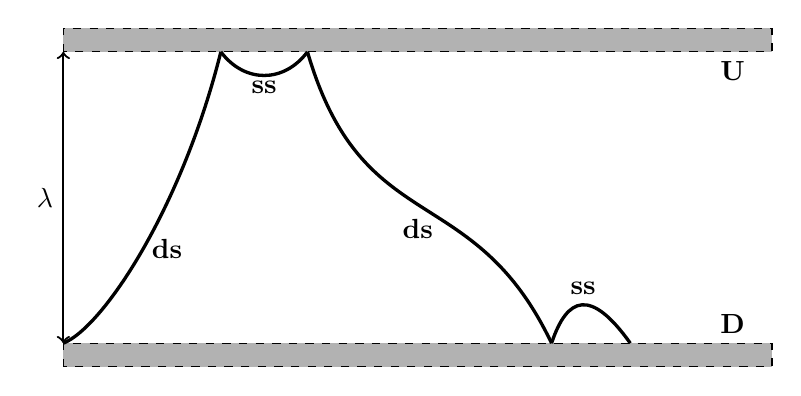
\begin{tikzpicture}
\usetikzlibrary{arrows}
\draw[fill=gray!60,dashed] (-3,0) rectangle (6,0.3);
\draw[fill=gray!60,dashed] (-3,-4) rectangle (6,-3.7);
\draw[very thick] (-3,-3.7) .. controls (-2.5,-3.5) and (-1.5,-2) .. (-1,0);
\draw[very thick] (-1,0) .. controls (-0.7,-0.4) and (-0.2,-0.4) .. (0.1,0);
\draw[very thick] (0.1,0) .. controls (0.8,-2.4) and (2.2,-1.6) .. (3.2,-3.7);
\draw[very thick] (3.2,-3.7) .. controls (3.4,-3.1) and (3.7,-3.0) .. (4.2,-3.7);
\draw (5.5,-3.7) node (d) [above] {$\mathbf{D}$};
\draw (5.5,0) node (u) [below] {$\mathbf{U}$};
\draw (-2.0,-2.5) node (ds1) [right] {$\mathbf{ds}$};
\draw (-0.45,-0.25) node (ss1) [below] {$\mathbf{ss}$};
\draw (1.5,-2) node (ds2) [below] {$\mathbf{ds}$};
\draw (3.6,-3.2) node (ss2) [above] {$\mathbf{ss}$};
%\draw [dashed,thick] (0,0.8) node (zaxis) [above] {$\mathbf{z}$}
%        |- (0.8,0) node (yaxis) [right] {$\mathbf{y}$};
\draw [<-,thick] (-3.,-3.7) -- (-3,-1.85) node (d) [left] {$\mathbf{\lambda}$};
\draw [<-,thick] (-3,0) -- (-3,-1.85);
\end{tikzpicture}
}
\end{center}
\caption{ A full scenario of electron's trajectories between parallel plates, including both double surface (ds) and single surface (ss) impacts. \cite{NS}\label{fig:ss-ds}}
\end{figure}

As described in \cite{NS}, the nonstationary statistical theory also starts from the equation of motion \eqref{vec}, and if we define $\xi=\omega z/v_{\omega}$, equation \eqref{position} can be rewritten by using this new variable as:
\begin{equation}
\xi(\varphi,\varphi_0,u) = (u+\cos \varphi_0)(\varphi-\varphi_0)+\sin \varphi_0 - \sin \varphi.\label{nposition}
\end{equation}
This equation describes the normalized position at phase $\varphi$, with starting phase $\varphi_0$ and initial velocity $u$. Following the definitions in nonstationary theory, each plate will be denoted as $D$ and $U$ for the boundary condition $\xi=0$ (down) and $\xi=\lambda$ (up), respectively. Double and single surface impacts with $D-U$ or $U-D$ and $D-D$ or $U-U$ trajectories will be denoted as $ds$ and $ss$ respectively. Other definitions for the nonstationary theory are given in \cite{NS}, and listed here in Table \ref{my_table} for convenience.
\begin{table}[h]\footnotesize
{\renewcommand{\arraystretch}{1.5}
\renewcommand{\tabcolsep}{0.2cm}}
\caption{Nonstationary theory definitions.}
\centering
  \label{my_table}
  \begin{tabular}{ l  r  }
    \hline
\hline			
    Impact rate (electrons/radian) in plate $U/D$ at phase $\varphi$ & $I_{U/D}(\varphi)$ \\
    Emission rate (electrons/radian) in plate $U/D$ at phase $\varphi$ & $C_{U/D}(\varphi)$ \\
    Number of electrons at time $\varphi$ & $N(\varphi)$ \\
    Probability density that an electron starting at plate $U/D$,\\
    with starting phase $\varphi$, experiences a double/single\\
    surface impact in a transit phase $\tau$ & $G_{ds/ss,U/D}(\tau|\varphi)$\\
    SEY of an electron starting at plate $U/D$, with starting\\
    phase $\varphi$, experiences a double/single surface impact\\
    in a transit phase $\tau$ & $\sigma_{ds/ss,U/D}(\tau|\varphi)$\\

    \hline 
 \hline
  \end{tabular}
 \end{table}

According to Vdovicheva et al. \cite{ST}, the joint probability density $G(\tau|\varphi_0;\lambda)$ is defined as
\begin{equation}
G(\tau|\varphi_0;\lambda)=\left| \frac{\mathrm{d}g(\tau|\varphi_0;\lambda)}{\mathrm{d}\tau} \right| f_u[g(\tau|\varphi_0;\lambda)] \label{gdsdef}
\end{equation}
where $u=g(\tau|\varphi_0;\lambda)$ should be a monotonic function, and is  obtained by working out $u$ from equation \eqref{pimpact} and removing the non-monotonic intervals. The detailed process to obtain $g(\tau|\varphi_0;\lambda)$ and consequently $G(\tau|\varphi_0;\lambda)$ is given in \cite{ST}.

To model the single surface impacts, the nonstationary theory use the joint probability density $G(\tau|\varphi_0;0)$ that the probability density of an electron starting at plate $U/D$, with starting phase $\varphi_0$, experiences single surface impact in a transit phase $\tau$ defined by
\begin{equation}
G(\tau|\varphi_0;0)=\left| \frac{\mathrm{d}g(\tau|\varphi_0;0)}{\mathrm{d}\tau} \right| f_u[g(\tau|\varphi_0;0)] \label{gssdef}
\end{equation}
where the $u=g(\tau|\varphi_0;0)$ is obtained by working out $u$ from equation \eqref{nposition} with an additional condition that $\xi=0$ (and removing the non-monotonic intervals).

As described in the stationary and nonstationary theory, not all the ejection velocity $u$ can be favorable for double or single surface impacts. There exists minimum $g(\tau|\varphi_0;\lambda)$ and maximum $g(\tau|\varphi_0;0)$ \cite{NS,ST} :  
\begin{align*}
 min\{g(\tau|\varphi_0;\lambda)\}=u_{min}\\
 max\{g(\tau|\varphi_0;0)\}=u_{max}
\end{align*}
where $u_{min}=u_{max}$ holds for the same starting phase $\varphi_0$. After setting up the joint probability density $G(\tau|\varphi_0;\lambda)$ and $G(\tau|\varphi_0;0)$, other definitions in Table \ref{my_table} will be given as follows \cite{NS} :
\begin{flalign}
C_U(\varphi)=&\int_0^\varphi C_D(\varphi')G_{ds,D}(\varphi-\varphi'|\varphi')\sigma_{ds,D}(\varphi-\varphi'|\varphi')\mathrm{d}\varphi'\nonumber \\
&+\int_0^\varphi C_U(\varphi')G_{ss,U}(\varphi-\varphi'|\varphi')\sigma_{ss,U}(\varphi-\varphi'|\varphi')\mathrm{d}\varphi'+\Psi_U(\varphi)\label{cudef}
\end{flalign}

\begin{flalign}
C_D(\varphi)=&\int_0^\varphi C_D(\varphi')G_{ss,D}(\varphi-\varphi'|\varphi')\sigma_{ss,D}(\varphi-\varphi'|\varphi')\mathrm{d}\varphi'\nonumber \\
&+\int_0^\varphi C_U(\varphi')G_{ds,U}(\varphi-\varphi'|\varphi')\sigma_{ds,U}(\varphi-\varphi'|\varphi')\mathrm{d}\varphi'+\Psi_D(\varphi)\label{cddef}
\end{flalign}

\begin{flalign}
I_U(\varphi)=&\int_0^\varphi C_D(\varphi')G_{ds,D}(\varphi-\varphi'|\varphi')\mathrm{d}\varphi'\nonumber \\
&+\int_0^\varphi C_U(\varphi')G_{ss,U}(\varphi-\varphi'|\varphi')\mathrm{d}\varphi'\label{iudef}
\end{flalign}

\begin{flalign}
I_D(\varphi)=&\int_0^\varphi C_D(\varphi')G_{ss,D}(\varphi-\varphi'|\varphi')\mathrm{d}\varphi'\nonumber \\
&+\int_0^\varphi C_U(\varphi')G_{ds,U}(\varphi-\varphi'|\varphi')\mathrm{d}\varphi'\label{iddef}
\end{flalign}

\begin{flalign}
N(\varphi)=&\int_0^\varphi \left(C_U(\varphi')+C_D(\varphi')-I_U(\varphi')-I_D(\varphi')\right)\mathrm{d}\varphi'\label{npdef}
\end{flalign}
where $\Psi_U(\varphi)$ and $\Psi_D(\varphi)$ are external electron sources from plate U and plate D, respectively, and the SEY $\sigma_{ds,D}(\varphi-\varphi'|\varphi')$, $\sigma_{ds,U}(\varphi-\varphi'|\varphi')$, $\sigma_{ss,D}(\varphi-\varphi'|\varphi')$, $\sigma_{ss,U}(\varphi-\varphi'|\varphi')$ can be converted to impact velocity related counterparts following the process in reference \cite{ST}.

For the theoretical model, the external source $\Psi_U(\varphi)=\Psi_D(\varphi)=1/2\delta(\varphi)$, where $\delta(\varphi)$ is the Dirac delta function. The SEY curve of copper provided in reference \cite{SE} to benchmark the Furman-Pivi model and the SEY curve of silver given in \cite{NS,FE} in order to benchmark Vaughan's  secondary emission model, (equation \eqref{cudef}, \eqref{cddef}).

The instantaneous SEY can be defined as:
\begin{equation}
\sigma_i=\frac{C(\varphi)}{I(\varphi)} \label{isey}
\end{equation}
The emission speed in the theoretical model follows the Maxwellian distribution\cite{NS}, 
\begin{equation}
f_u=\frac{uv^2_{\omega}}{v^2_t}\exp{\left(-\frac{u^2v^2_{\omega}}{2v^2_t}\right)}.\label{maxwellian}
\end{equation}


\section{Matlab scripts for reproducing the above theory}
\subsection{Scripts used for reproducing monotonic velocity function}
According to \cite{NS}, for each initial phase $\varphi_{s}\in [0: 2\pi : \pi/180)$, the minimum ejection velocity for double surface is equal to the maximum ejection velocity for single surface, i.e., $min(u_{ds})=max(u_{ss})$. We need to reproduce this by running script ``$\mathbf{umin.m}$". You can edit this script to change voltage, frequency and distance (maybe also the thermal velocity of emission particles) between parallel plates. The places where we can change those parameters are documented within that script. Running the script ``$\mathbf{umin.m}$" will generate a data file ``$\mathbf{umin.txt}$" which contains the initial phase $\varphi_{s}\in [0: 2\pi : \pi/180)$ (in the first column), the value of $min(u_{ds})=max(u_{ss})$ (second column) and the none units time $\mathbf{\tau}$ when the monotonic velocity function reaches the minimum or maximum velocity.

Then run the ``$\mathbf{uss\_coeff\_.m}$" and ``$\mathbf{uds\_coeff\_.m}$" to get the none units time interval of the none monotonic candidate velocity function
(working out $u$ from \eqref{pimpact}) according to its stationary points and build none units time interval lookup table for each initial phase $\varphi_{s}\in [0: 2\pi : \pi/180)$. There are two lookup tables, i.e., ``$\mathbf{uds\_coeff.txt}$" and ``$\mathbf{uss\_coeff.txt}$" relative to double surface impact and single surface impact respectively. Open the  ``$\mathbf{uds\_coeff.txt}$" and ``$\mathbf{uss\_coeff.txt}$", if they are all correct, then change the file names to ``$\mathbf{myuds\_coeff.txt}$" and  ``$\mathbf{myuss\_coeff.txt}$" respectively. The file ``$\mathbf{myuds\_coeff.txt}$" contains the initial phase (the first column) and the time intervals. The ``$\mathbf{myuss\_coeff.txt}$" contains only initial phase (the first column) and the none units time when the $u_{ss}$ reaches its maximum.

After building the necessary coefficients needed by monotonic velocity function, we can test the validation of monotonic function by run ``$\mathbf{plot\_monotonic.m}$" to see the resulting monotonic velocity functions.

For the case of Vaughan's model with the same parameter as in \cite{NS}, we can also run ``$\mathbf{reproduce6.m}$" to get figure 6 of reference \cite{NS}.

Then run the ``$\mathbf{reproduce8.m}$" to calculate the time evolution of particles. ``$\mathbf{reproduce8.m}$" will automatically invoke the script ``$\mathbf{seedg.m}$" to get external electron source and the script ``$\mathbf{ak.m}$" to build the core of Volterra integral in \eqref{cudef} and \eqref{cddef}. 

The script ``$\mathbf{ak.m}$" will automatically invoke the scripts ``$\mathbf{mygss\_u.m}$", ``$\mathbf{seyss\_u.m}$", ``$\mathbf{ mygds\_d.m}$", ``$\mathbf{seyds\_d.m}$", ``$\mathbf{mygds\_u.m}$", ``$\mathbf{seyds\_u.m}$", ``$\mathbf{mygss\_d.m}$", ``$\mathbf{seyss\_d.m}$" to build correct monotonic velocity function for single/double surface impact and SEY expressions.

The time evolution data is stored in ``$\mathbf{fig8\_result.txt}$", you can either use gnuplot or matlab to plot the data.
And one of the side results, the time evolution of instantaneous SEY, can be ploted by script $\mathbf{SEY\_plot.m}$, according to equation \eqref{isey}. 
\begin{thebibliography}{99}
\bibitem{SE} M. A. Furman and M. T. F. Pivi,  
Phys. Rev. ST Accel. Beams 5, 124404 (2002)
\bibitem{VH} J. Rodney M. Vaughan, IEEE Transactions on Electron Devices. Vol. 36, No. 9, September 1989
\bibitem{FE} C. Vicente, M. Mattes, D. Wolk, H. L. Hartnagel, J. R. Mosig, D. Raboso, Proc. MULCOPIM 2005, ESTEC-ESA, Noordwijk, The Netherlands, 2005, pp. 11-17
\bibitem{PP} A. Kryazhev, M. Buyanova, V. Semenov, D. Anderson and M. Lisak, J. Puech, L. Lapierre, and J. Sombrin,
Phys. Plasmas, Vol. 9, No. 11, November 2002
\bibitem{PN} R. Udiljak, D. Anderson, and M. Lisak, V. E. Semenov, J. Puech, Phys. Plasmas 14, 033508 2007
\bibitem{NS} S. Anza, C. Vicente, J. Gil, V. E. Boria, B. Gimeno, and D. Raboso, Phys. Plasmas 17, 062110 2010
\bibitem{ST} N. K. Vdovicheva, A. G. Sazontov, and V. E. Semenov, Radiophys. Quantum Electron. 47, 580 2004.

\end{thebibliography} 
\end{document}


% LocalWords:  Anylitical
